\documentclass[11pt]{article}
\usepackage{mathtools,hyperref,booktabs,fullpage, txfonts}
\usepackage[amssymb,cdot]{SIunits}
\usepackage[utopia]{mathdesign}     

\usepackage[table]{xcolor}
\usepackage{amsmath}
\usepackage{hyperref}
\usepackage{longtable}
\usepackage{fullpage}
 
\definecolor{lightgray}{gray}{0.93}

\pagestyle{empty}
\setlength\parindent{0pt}
\renewcommand{\thefootnote}{\fnsymbol{footnote}}
 
\makeatletter
\renewcommand\section{\@startsection{section}{1}{\z@}%
                                  {-3.5ex \@plus -1ex \@minus -.2ex}%
                                  {2.3ex \@plus.2ex}%
                                  {\normalfont\bfseries}}
\makeatother


\begin{document}

\subsection*{Brendan Ward - 9/1}

{\large
  \begin{center}
    {\bf          Homework 1 }
  \end{center}
}
 

\section*{Problem 1 -- More in the Command Line}

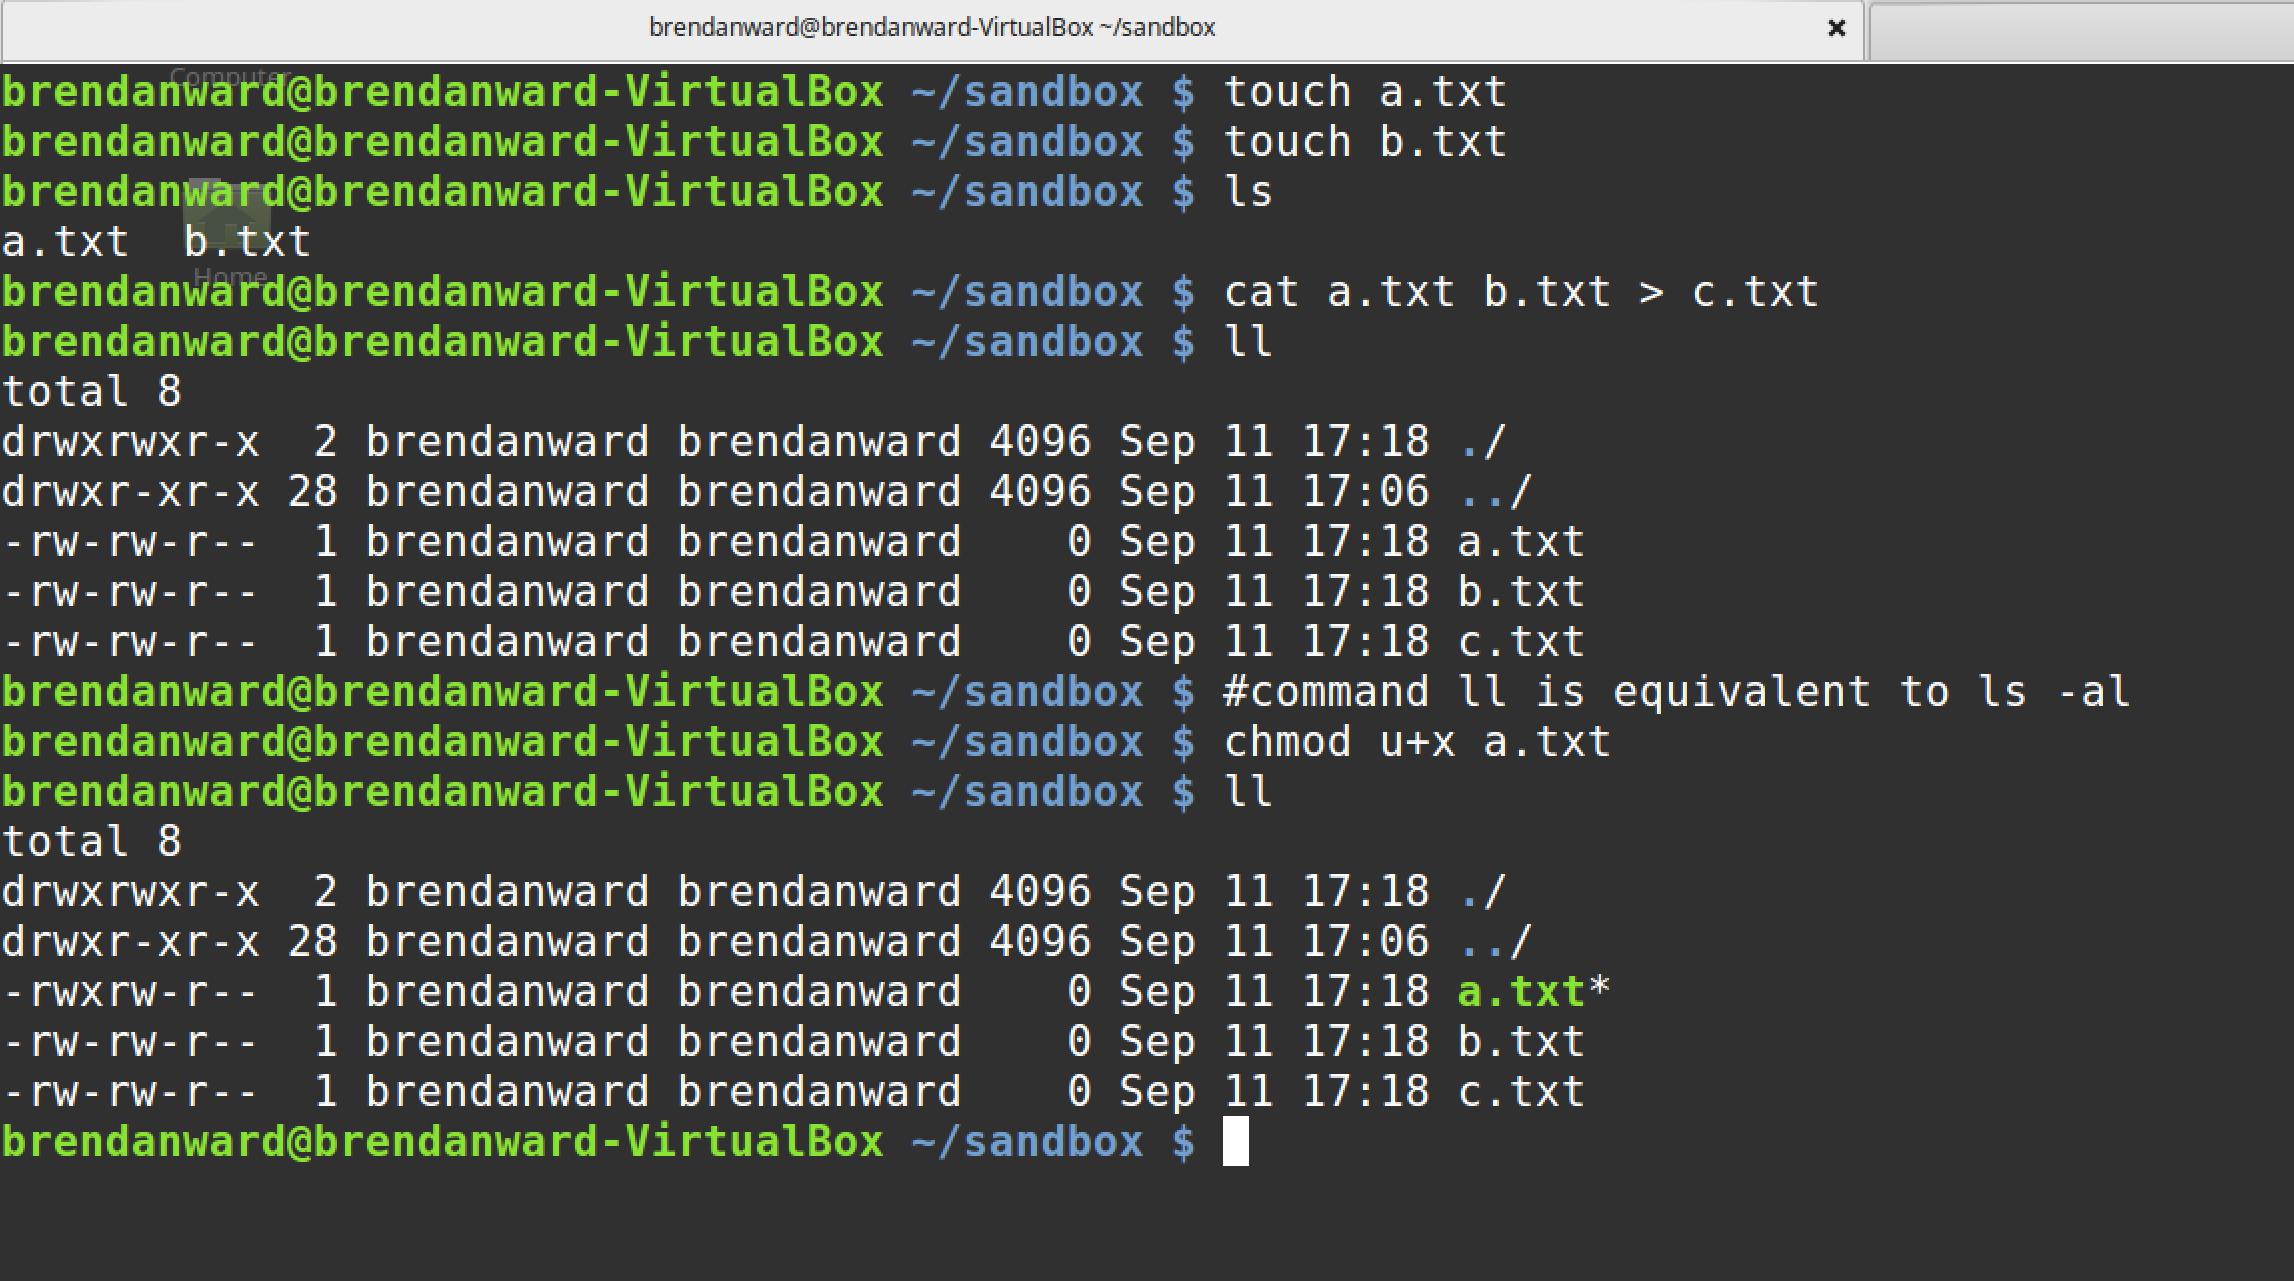
\includegraphics[width=\textwidth]{HW2_1.png}

\section*{Problem 2 -- Simple Shell Scripting -- Files located in GitHub repository}
 
\begin{enumerate}
\item FtoC.sh
\item countcd.sh
\item move2trash.sh
\end{enumerate}

\section*{Problem 3 -- Git and Version Control}

\begin{enumerate}
 \item Get a (free) account at GitHub  and create a 
       repository for your shell scripts.  
       Provide me a link to this repository so I can see it.
 \item Modify the temperature conversion script to output the 
       temperature in Kelvin, too, and use 
       use {\tt git} (and GitHub, etc.) to track this change.
\end{enumerate}
 


\end{document}
